% Options for packages loaded elsewhere
\PassOptionsToPackage{unicode}{hyperref}
\PassOptionsToPackage{hyphens}{url}
%
\documentclass[
  ignorenonframetext,
]{beamer}
\usepackage{pgfpages}
\setbeamertemplate{caption}[numbered]
\setbeamertemplate{caption label separator}{: }
\setbeamercolor{caption name}{fg=normal text.fg}
\beamertemplatenavigationsymbolsempty
% Prevent slide breaks in the middle of a paragraph
\widowpenalties 1 10000
\raggedbottom
\setbeamertemplate{part page}{
  \centering
  \begin{beamercolorbox}[sep=16pt,center]{part title}
    \usebeamerfont{part title}\insertpart\par
  \end{beamercolorbox}
}
\setbeamertemplate{section page}{
  \centering
  \begin{beamercolorbox}[sep=12pt,center]{part title}
    \usebeamerfont{section title}\insertsection\par
  \end{beamercolorbox}
}
\setbeamertemplate{subsection page}{
  \centering
  \begin{beamercolorbox}[sep=8pt,center]{part title}
    \usebeamerfont{subsection title}\insertsubsection\par
  \end{beamercolorbox}
}
\AtBeginPart{
  \frame{\partpage}
}
\AtBeginSection{
  \ifbibliography
  \else
    \frame{\sectionpage}
  \fi
}
\AtBeginSubsection{
  \frame{\subsectionpage}
}
\usepackage{amsmath,amssymb}
\usepackage{lmodern}
\usepackage{iftex}
\ifPDFTeX
  \usepackage[T1]{fontenc}
  \usepackage[utf8]{inputenc}
  \usepackage{textcomp} % provide euro and other symbols
\else % if luatex or xetex
  \usepackage{unicode-math}
  \defaultfontfeatures{Scale=MatchLowercase}
  \defaultfontfeatures[\rmfamily]{Ligatures=TeX,Scale=1}
\fi
% Use upquote if available, for straight quotes in verbatim environments
\IfFileExists{upquote.sty}{\usepackage{upquote}}{}
\IfFileExists{microtype.sty}{% use microtype if available
  \usepackage[]{microtype}
  \UseMicrotypeSet[protrusion]{basicmath} % disable protrusion for tt fonts
}{}
\makeatletter
\@ifundefined{KOMAClassName}{% if non-KOMA class
  \IfFileExists{parskip.sty}{%
    \usepackage{parskip}
  }{% else
    \setlength{\parindent}{0pt}
    \setlength{\parskip}{6pt plus 2pt minus 1pt}}
}{% if KOMA class
  \KOMAoptions{parskip=half}}
\makeatother
\usepackage{xcolor}
\newif\ifbibliography
\usepackage{color}
\usepackage{fancyvrb}
\newcommand{\VerbBar}{|}
\newcommand{\VERB}{\Verb[commandchars=\\\{\}]}
\DefineVerbatimEnvironment{Highlighting}{Verbatim}{commandchars=\\\{\}}
% Add ',fontsize=\small' for more characters per line
\usepackage{framed}
\definecolor{shadecolor}{RGB}{248,248,248}
\newenvironment{Shaded}{\begin{snugshade}}{\end{snugshade}}
\newcommand{\AlertTok}[1]{\textcolor[rgb]{0.94,0.16,0.16}{#1}}
\newcommand{\AnnotationTok}[1]{\textcolor[rgb]{0.56,0.35,0.01}{\textbf{\textit{#1}}}}
\newcommand{\AttributeTok}[1]{\textcolor[rgb]{0.77,0.63,0.00}{#1}}
\newcommand{\BaseNTok}[1]{\textcolor[rgb]{0.00,0.00,0.81}{#1}}
\newcommand{\BuiltInTok}[1]{#1}
\newcommand{\CharTok}[1]{\textcolor[rgb]{0.31,0.60,0.02}{#1}}
\newcommand{\CommentTok}[1]{\textcolor[rgb]{0.56,0.35,0.01}{\textit{#1}}}
\newcommand{\CommentVarTok}[1]{\textcolor[rgb]{0.56,0.35,0.01}{\textbf{\textit{#1}}}}
\newcommand{\ConstantTok}[1]{\textcolor[rgb]{0.00,0.00,0.00}{#1}}
\newcommand{\ControlFlowTok}[1]{\textcolor[rgb]{0.13,0.29,0.53}{\textbf{#1}}}
\newcommand{\DataTypeTok}[1]{\textcolor[rgb]{0.13,0.29,0.53}{#1}}
\newcommand{\DecValTok}[1]{\textcolor[rgb]{0.00,0.00,0.81}{#1}}
\newcommand{\DocumentationTok}[1]{\textcolor[rgb]{0.56,0.35,0.01}{\textbf{\textit{#1}}}}
\newcommand{\ErrorTok}[1]{\textcolor[rgb]{0.64,0.00,0.00}{\textbf{#1}}}
\newcommand{\ExtensionTok}[1]{#1}
\newcommand{\FloatTok}[1]{\textcolor[rgb]{0.00,0.00,0.81}{#1}}
\newcommand{\FunctionTok}[1]{\textcolor[rgb]{0.00,0.00,0.00}{#1}}
\newcommand{\ImportTok}[1]{#1}
\newcommand{\InformationTok}[1]{\textcolor[rgb]{0.56,0.35,0.01}{\textbf{\textit{#1}}}}
\newcommand{\KeywordTok}[1]{\textcolor[rgb]{0.13,0.29,0.53}{\textbf{#1}}}
\newcommand{\NormalTok}[1]{#1}
\newcommand{\OperatorTok}[1]{\textcolor[rgb]{0.81,0.36,0.00}{\textbf{#1}}}
\newcommand{\OtherTok}[1]{\textcolor[rgb]{0.56,0.35,0.01}{#1}}
\newcommand{\PreprocessorTok}[1]{\textcolor[rgb]{0.56,0.35,0.01}{\textit{#1}}}
\newcommand{\RegionMarkerTok}[1]{#1}
\newcommand{\SpecialCharTok}[1]{\textcolor[rgb]{0.00,0.00,0.00}{#1}}
\newcommand{\SpecialStringTok}[1]{\textcolor[rgb]{0.31,0.60,0.02}{#1}}
\newcommand{\StringTok}[1]{\textcolor[rgb]{0.31,0.60,0.02}{#1}}
\newcommand{\VariableTok}[1]{\textcolor[rgb]{0.00,0.00,0.00}{#1}}
\newcommand{\VerbatimStringTok}[1]{\textcolor[rgb]{0.31,0.60,0.02}{#1}}
\newcommand{\WarningTok}[1]{\textcolor[rgb]{0.56,0.35,0.01}{\textbf{\textit{#1}}}}
\usepackage{graphicx}
\makeatletter
\def\maxwidth{\ifdim\Gin@nat@width>\linewidth\linewidth\else\Gin@nat@width\fi}
\def\maxheight{\ifdim\Gin@nat@height>\textheight\textheight\else\Gin@nat@height\fi}
\makeatother
% Scale images if necessary, so that they will not overflow the page
% margins by default, and it is still possible to overwrite the defaults
% using explicit options in \includegraphics[width, height, ...]{}
\setkeys{Gin}{width=\maxwidth,height=\maxheight,keepaspectratio}
% Set default figure placement to htbp
\makeatletter
\def\fps@figure{htbp}
\makeatother
\setlength{\emergencystretch}{3em} % prevent overfull lines
\providecommand{\tightlist}{%
  \setlength{\itemsep}{0pt}\setlength{\parskip}{0pt}}
\setcounter{secnumdepth}{-\maxdimen} % remove section numbering
\ifLuaTeX
  \usepackage{selnolig}  % disable illegal ligatures
\fi
\IfFileExists{bookmark.sty}{\usepackage{bookmark}}{\usepackage{hyperref}}
\IfFileExists{xurl.sty}{\usepackage{xurl}}{} % add URL line breaks if available
\urlstyle{same} % disable monospaced font for URLs
\hypersetup{
  pdftitle={Cournot Nash Equilibrium},
  pdfauthor={Marly Tatiana Celis},
  hidelinks,
  pdfcreator={LaTeX via pandoc}}

\title{Cournot Nash Equilibrium}
\subtitle{Industrial Organization and Competition Policy}
\author{Marly Tatiana Celis}
\date{December 7th, 2023}

\begin{document}
\frame{\titlepage}

\begin{frame}{Cournot Market Structure}
\protect\hypertarget{cournot-market-structure}{}
This is a simple code for representing the Cournot equilibrium for a
duopoly when market demand is \(Q(P)=200-P\). Each firm's cost function
is \(C(q_i )=20q_i\), where \(i=1,2\).

\begin{itemize}
\item
  In this case the Cournot model corresponds to two firms with symmetric
  costs.
\item
  Each firm's goal is to chose the level of output that maximizes
  profits, given the output of the other firm.
\item
  Firm i's payoffs are profits \(\pi_i(q_i,q_j)=(p-c)q_i\)
\end{itemize}
\end{frame}

\begin{frame}[fragile]{Create data frame with output values for each
firm}
\protect\hypertarget{create-data-frame-with-output-values-for-each-firm}{}
The first step consist on creating a data frame with two columns. On
column for the output for firm 1 and another column with the output for
firm 2.

Next, we create some value with the parameters of the demand and costs
functions.

\begin{Shaded}
\begin{Highlighting}[]
\FunctionTok{rm}\NormalTok{(}\AttributeTok{list=}\FunctionTok{ls}\NormalTok{())}

\CommentTok{\# Create output q and define the range of values}
\NormalTok{cournotdata }\OtherTok{\textless{}{-}} \FunctionTok{data.frame}\NormalTok{(}\AttributeTok{output\_firm1 =} \FunctionTok{seq}\NormalTok{(}\DecValTok{0}\NormalTok{, }\DecValTok{180}\NormalTok{, }\AttributeTok{by =} \DecValTok{10}\NormalTok{),}
                 \AttributeTok{output\_firm2 =} \FunctionTok{seq}\NormalTok{(}\DecValTok{0}\NormalTok{, }\DecValTok{180}\NormalTok{, }\AttributeTok{by =} \DecValTok{10}\NormalTok{))}

\CommentTok{\# Create values with parameters of the functions }
\NormalTok{a }\OtherTok{\textless{}{-}} \DecValTok{200}
\NormalTok{c }\OtherTok{\textless{}{-}} \DecValTok{20}
\NormalTok{b }\OtherTok{\textless{}{-}} \DecValTok{1}
\end{Highlighting}
\end{Shaded}
\end{frame}

\begin{frame}{Nash equilibrium}
\protect\hypertarget{nash-equilibrium}{}
At the Nash equilibrium, recall that each firm must behave optimally
assuming that its rival b ehaves optimally. That is, firm \(i\)
maximizes profits , believing that firm \(j\) maximizes its profits.
Another way of saying this is that each firm calculates its best
response or reply to the expected best-reply behavior of the other firm

\(q_1=\frac{a-c-bq_2}{2b}\)

\(q_2=\frac{a-c-bq_1}{2b}\)
\end{frame}

\begin{frame}[fragile]{Compute best responses}
\protect\hypertarget{compute-best-responses}{}
\begin{Shaded}
\begin{Highlighting}[]
\CommentTok{\# Compute best responses}
\NormalTok{cournotdata }\OtherTok{\textless{}{-}}\NormalTok{ cournotdata }\SpecialCharTok{\%\textgreater{}\%} 
  \FunctionTok{mutate}\NormalTok{( }\AttributeTok{bestresp\_Firm1 =}\NormalTok{ (a}\SpecialCharTok{{-}}\NormalTok{c}\SpecialCharTok{{-}}\NormalTok{b}\SpecialCharTok{*}\NormalTok{output\_firm2)}\SpecialCharTok{*}\NormalTok{((}\DecValTok{2}\SpecialCharTok{*}\NormalTok{b)}\SpecialCharTok{\^{}{-}}\DecValTok{1}\NormalTok{),}
          \AttributeTok{bestresp\_Firm2 =}\NormalTok{ (a}\SpecialCharTok{{-}}\NormalTok{c}\SpecialCharTok{{-}}\NormalTok{b}\SpecialCharTok{*}\NormalTok{output\_firm1)}\SpecialCharTok{*}\NormalTok{((}\DecValTok{2}\SpecialCharTok{*}\NormalTok{b)}\SpecialCharTok{\^{}{-}}\DecValTok{1}\NormalTok{)}
\NormalTok{          )}

\FunctionTok{ggplot}\NormalTok{() }\SpecialCharTok{+}
  \FunctionTok{geom\_line}\NormalTok{(}\AttributeTok{data =}\NormalTok{ cournotdata, }\FunctionTok{aes}\NormalTok{(}\AttributeTok{x =}\NormalTok{ output\_firm1, }\AttributeTok{y =}\NormalTok{ bestresp\_Firm2), }\AttributeTok{color =} \StringTok{"blue"}\NormalTok{, }\AttributeTok{size =} \FloatTok{1.5}\NormalTok{) }\SpecialCharTok{+}
  \FunctionTok{geom\_line}\NormalTok{(}\AttributeTok{data =}\NormalTok{ cournotdata, }\FunctionTok{aes}\NormalTok{(}\AttributeTok{x =}\NormalTok{ bestresp\_Firm1, }\AttributeTok{y =}\NormalTok{ output\_firm2), }\AttributeTok{color =} \StringTok{"red"}\NormalTok{, }\AttributeTok{size =} \FloatTok{1.5}\NormalTok{) }\SpecialCharTok{+}
  \FunctionTok{labs}\NormalTok{(}\AttributeTok{title =} \StringTok{"Best Responses"}\NormalTok{, }\AttributeTok{x =} \StringTok{"Output Firm 1"}\NormalTok{, }\AttributeTok{y =} \StringTok{"Output Firm 2"}\NormalTok{) }\SpecialCharTok{+}
  \FunctionTok{scale\_x\_continuous}\NormalTok{(}\AttributeTok{breaks =} \FunctionTok{seq}\NormalTok{(}\DecValTok{0}\NormalTok{, }\FunctionTok{max}\NormalTok{(cournotdata}\SpecialCharTok{$}\NormalTok{output\_firm1, cournotdata}\SpecialCharTok{$}\NormalTok{bestresp\_Firm1), }\AttributeTok{by =} \DecValTok{20}\NormalTok{)) }\SpecialCharTok{+}
  \FunctionTok{scale\_y\_continuous}\NormalTok{(}\AttributeTok{breaks =} \FunctionTok{seq}\NormalTok{(}\DecValTok{0}\NormalTok{, }\FunctionTok{max}\NormalTok{(cournotdata}\SpecialCharTok{$}\NormalTok{output\_firm1, cournotdata}\SpecialCharTok{$}\NormalTok{bestresp\_Firm1), }\AttributeTok{by =} \DecValTok{20}\NormalTok{)) }\SpecialCharTok{+}
  \FunctionTok{theme\_minimal}\NormalTok{()}
\end{Highlighting}
\end{Shaded}

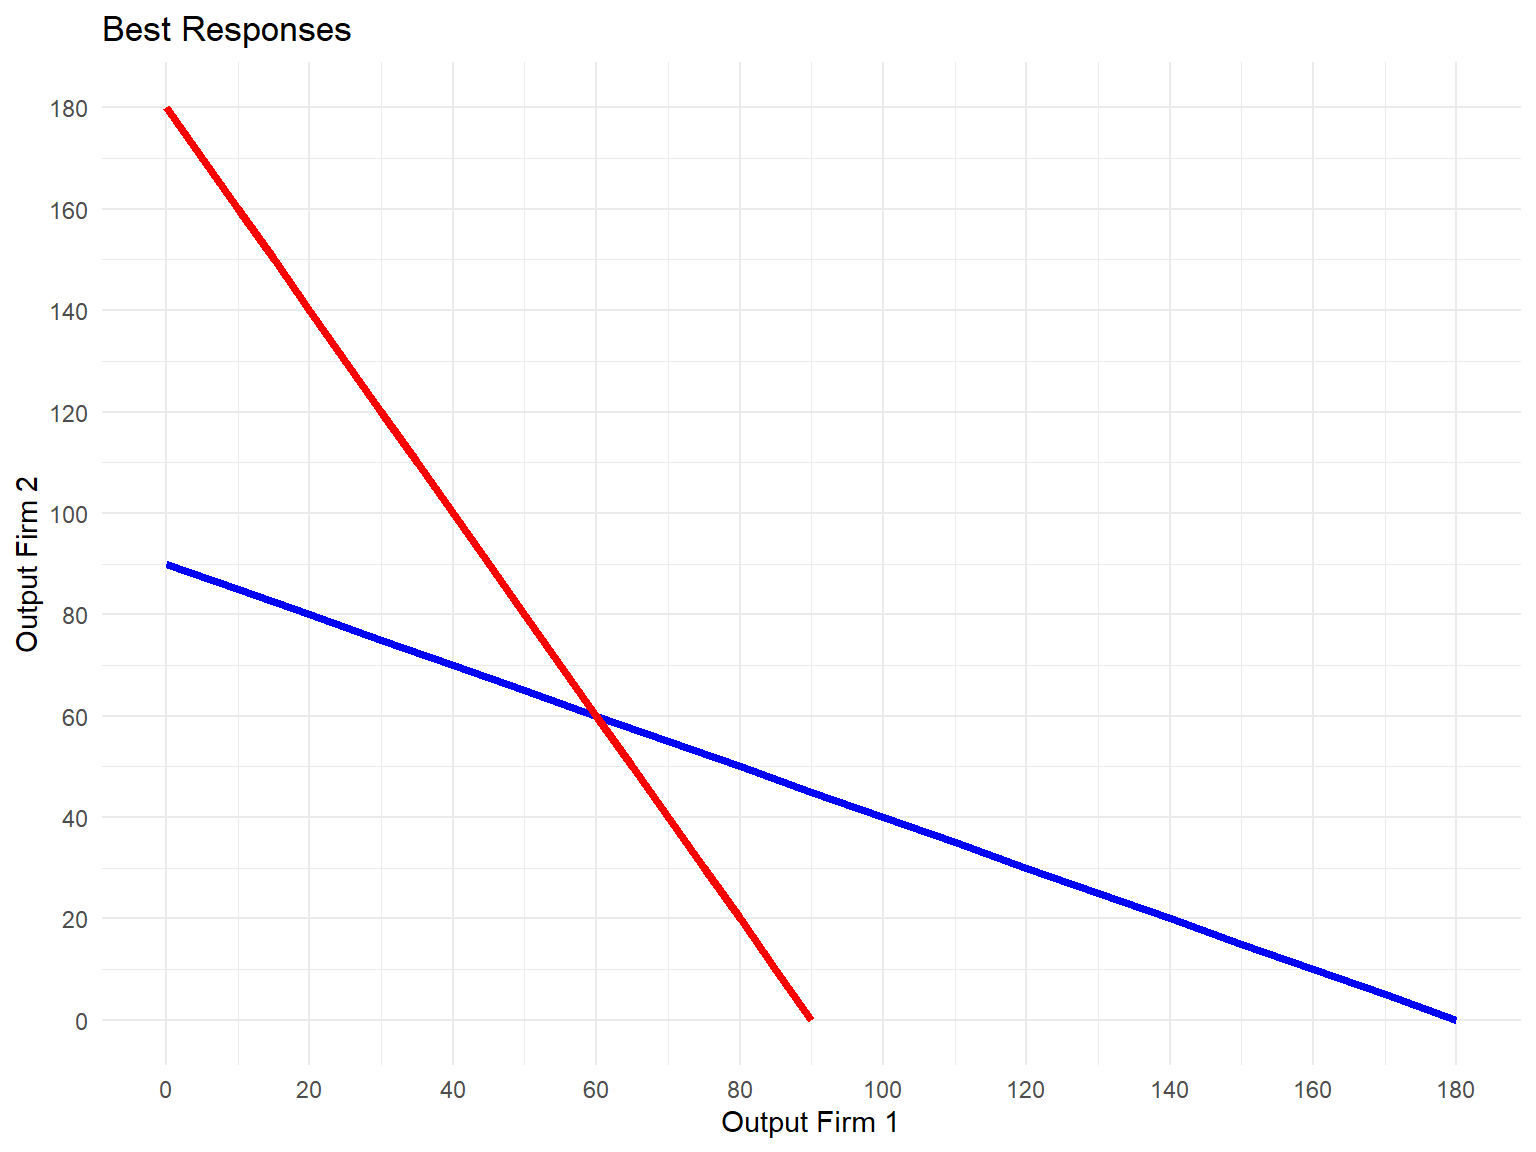
\includegraphics{cournot_graph_files/figure-beamer/cournot data-1.pdf}
\end{frame}

\begin{frame}[fragile]{Compute equilibrium}
\protect\hypertarget{compute-equilibrium}{}
Solving simultaneaously for \(q_1\) and \(q_2\) we get

\(q_1 =\frac{a-c}{3b}\)

\(q_2 =\frac{a-c}{3b}\)

Compute best responses

\begin{Shaded}
\begin{Highlighting}[]
\CommentTok{\# Compute best responses}

\NormalTok{nashoutput\_firm1}\OtherTok{=}\NormalTok{ (a}\SpecialCharTok{{-}}\NormalTok{c)}\SpecialCharTok{*}\NormalTok{((}\DecValTok{3}\SpecialCharTok{*}\NormalTok{b)}\SpecialCharTok{\^{}{-}}\DecValTok{1}\NormalTok{)}
\NormalTok{nashoutput\_firm2}\OtherTok{=}\NormalTok{ (a}\SpecialCharTok{{-}}\NormalTok{c)}\SpecialCharTok{*}\NormalTok{((}\DecValTok{3}\SpecialCharTok{*}\NormalTok{b)}\SpecialCharTok{\^{}{-}}\DecValTok{1}\NormalTok{)}

\FunctionTok{ggplot}\NormalTok{() }\SpecialCharTok{+}
  \FunctionTok{geom\_line}\NormalTok{(}\AttributeTok{data =}\NormalTok{ cournotdata, }\FunctionTok{aes}\NormalTok{(}\AttributeTok{x =}\NormalTok{ output\_firm1, }\AttributeTok{y =}\NormalTok{ bestresp\_Firm2), }\AttributeTok{color =} \StringTok{"blue"}\NormalTok{, }\AttributeTok{size =} \FloatTok{1.5}\NormalTok{) }\SpecialCharTok{+}
  \FunctionTok{geom\_line}\NormalTok{(}\AttributeTok{data =}\NormalTok{ cournotdata, }\FunctionTok{aes}\NormalTok{(}\AttributeTok{x =}\NormalTok{ bestresp\_Firm1, }\AttributeTok{y =}\NormalTok{ output\_firm2), }\AttributeTok{color =} \StringTok{"red"}\NormalTok{, }\AttributeTok{size =} \FloatTok{1.5}\NormalTok{) }\SpecialCharTok{+}
  \FunctionTok{labs}\NormalTok{(}\AttributeTok{title =} \StringTok{"Best Responses"}\NormalTok{, }\AttributeTok{x =} \StringTok{"Output Firm 1"}\NormalTok{, }\AttributeTok{y =} \StringTok{"Output Firm 2"}\NormalTok{) }\SpecialCharTok{+}
  \FunctionTok{geom\_point}\NormalTok{(}\FunctionTok{aes}\NormalTok{(}\AttributeTok{x =}\NormalTok{ nashoutput\_firm1, }\AttributeTok{y =}\NormalTok{ nashoutput\_firm2), }\AttributeTok{color =} \StringTok{"green"}\NormalTok{, }\AttributeTok{size =} \DecValTok{3}\NormalTok{) }\SpecialCharTok{+}  \CommentTok{\# Add the single point}
  \FunctionTok{scale\_x\_continuous}\NormalTok{(}\AttributeTok{breaks =} \FunctionTok{seq}\NormalTok{(}\DecValTok{0}\NormalTok{, }\FunctionTok{max}\NormalTok{(cournotdata}\SpecialCharTok{$}\NormalTok{output\_firm1, cournotdata}\SpecialCharTok{$}\NormalTok{bestresp\_Firm1), }\AttributeTok{by =} \DecValTok{20}\NormalTok{)) }\SpecialCharTok{+}
  \FunctionTok{scale\_y\_continuous}\NormalTok{(}\AttributeTok{breaks =} \FunctionTok{seq}\NormalTok{(}\DecValTok{0}\NormalTok{, }\FunctionTok{max}\NormalTok{(cournotdata}\SpecialCharTok{$}\NormalTok{output\_firm1, cournotdata}\SpecialCharTok{$}\NormalTok{bestresp\_Firm1), }\AttributeTok{by =} \DecValTok{20}\NormalTok{)) }\SpecialCharTok{+}
  \FunctionTok{theme\_minimal}\NormalTok{()}
\end{Highlighting}
\end{Shaded}

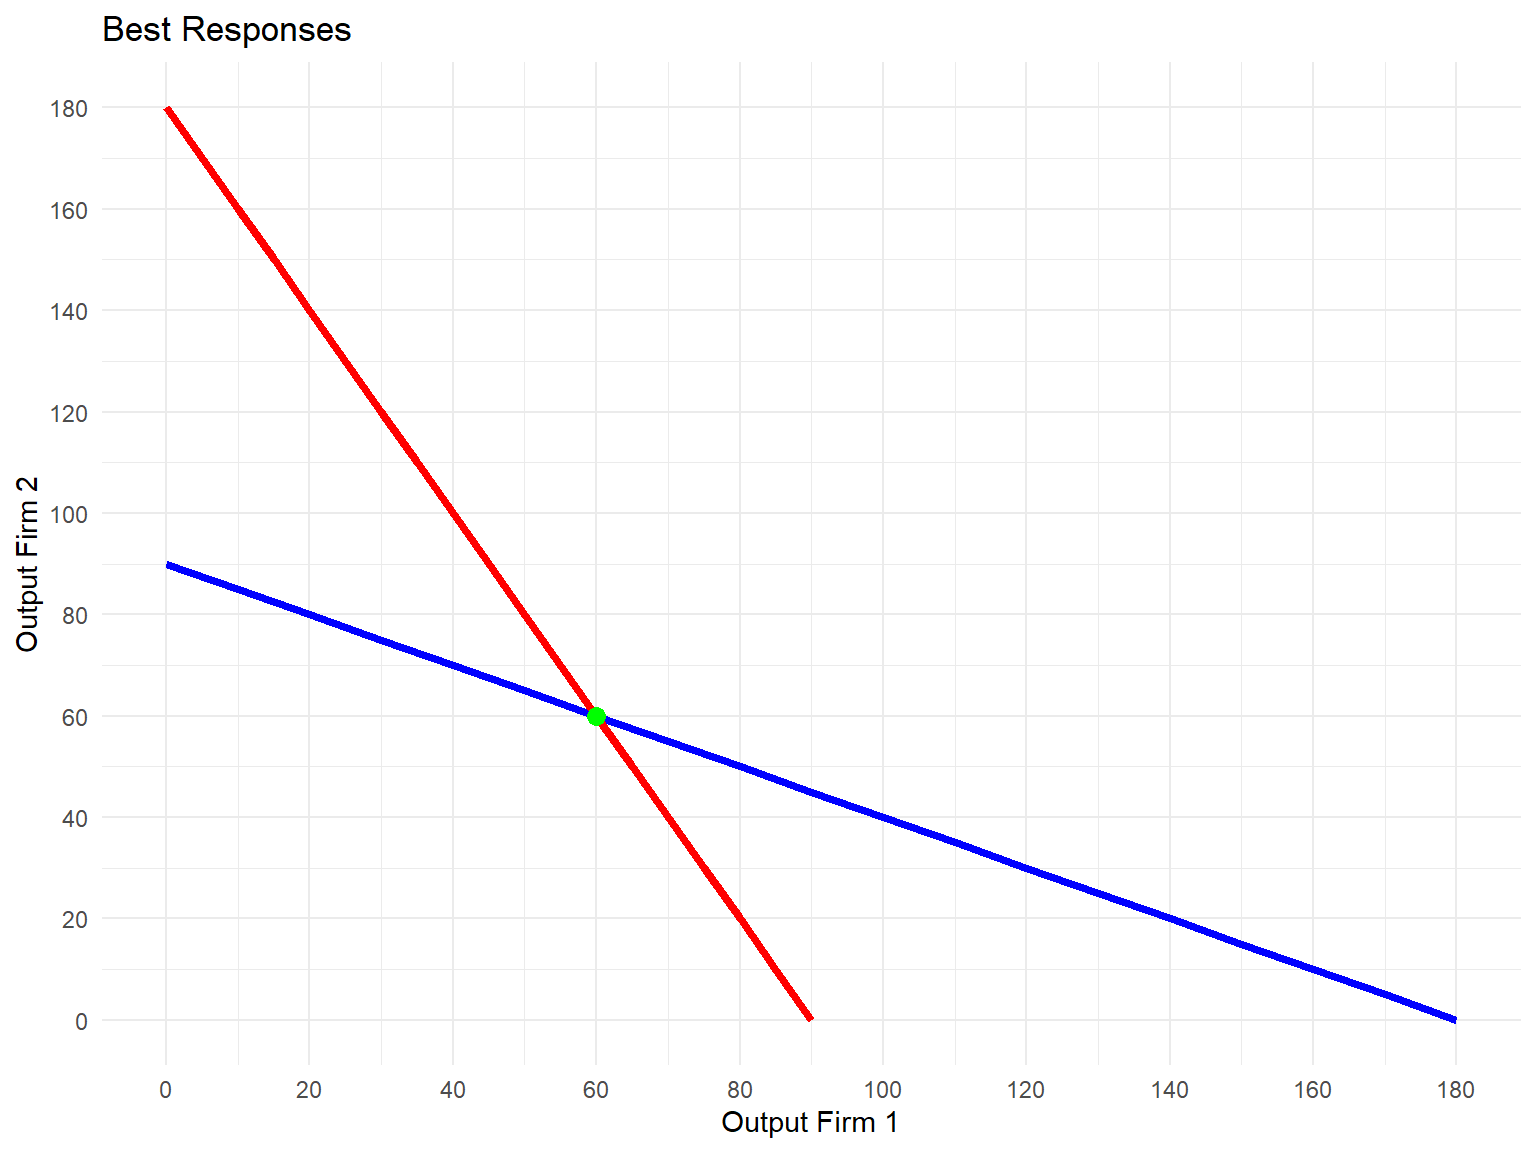
\includegraphics{cournot_graph_files/figure-beamer/cournot nash-1.pdf}
\end{frame}

\end{document}
